
\section{Evaluation}
\label{sec:Evaluation}
In the proposed two step for $\MyProblemAbrreviation$ problem, we employ a proactive failure dependent protection(FD) based $\MyProblemAbrreviation$ design with sufficient redundancy before embedding process in order to conquer the limitation of existing work, which consider the redundancy within the embedding process and failure independent protection based migration approach in resource efficiency.(Shared or nonShared)\cite{lu2006efficient}


In this section, we evaluate the performance of the SeVN heuristic method when allocating resources with considered all virtual nodes. In particular, we focus on the resource usage of the physical infrastructure and virtual network request, and the admission rates of eVN survivable requests. We further compare that to a virtual request where VN do not have survivability requirement, i.e.
virtual network request (labeled VN), as a baseline to gauge the additional amount of resources consumed for survivability.

current: every virtual network's request exist relative lease time, record current virtual or substrate network's performance in current situation.

Accumulate: additional record every virtual or substrate network's performance.

We first describe the simulation setup, then present the simulation results.
\subsection{Simulation Settings}
For any VN request, the number of VN nodes is randomly determined by a uniform distribution between $\VirtualNodeSizeMinimum$ and $\VirtualNodeSizeMaximum$ and each pair of virtual nodes is randomly connected with probability $\VirtualNodenodeProbability$. The computing requirements on VN nodes follow a uniform distribution from $\VirtualNodeComputationMinimum$ to $\VirtualNodeComputationMaximum$, as well as the bandwidth on VN links from $\VirtualEdgeBandwithMinimum$ to $\VirtualEdgeBandwithMaximum$.

VN requests arrive randomly over a timespan of $\SubstrateNewtorkRunTimeInterval$ time slots and the inter-arrival time is
assumed to follow the Geometric distribution at a rate of $\requestAppearProbability$ per time slot. The resource lease times of each VN follows the uniform distribution as well at a rate  range from $\VNRequestsContinueTimeMinimum$ and $\VNRequestsContinueTimeMaximum$ per time slot. A high request rate and long lease times ensures that the physical infrastructure is operating at high utilization.

We assume the relative cost of computing and bandwidth is $\RelativeCostbetweenComputingBandwidth$\cite{armbrust2009above,yu2010survivable}, which means $\theta=\RelativeCostbetweenComputingBandwidth$. The SN topologies used are randomly generated with $\SubStrateNodeSize$ nodes using random generating graph method. The computing(bandwidth) resources of the substrate nodes (links) are real numbers uniformly distributed between $\SubStrateNodeComputationMinimum$ and $\SubStrateNodeComputationMaximum$ ($\SubStrateEdgeBandwithMinimum$ and $\SubStrateEdgeBandwithMaximum$).
%To model the facility node failure scenario, we randomly choose one substrate facility node to fail in every $\SubStrateFacilityNodeFailDuration$ time units..
%the GT-ITM tool\cite{zegura1996model}

%The arrivals of VN requests are modeled by a Poisson process (with mean of 10 requests per 100 time units). The duration of the requests follows an exponential distribution with 1000 time units on average.

%The physical infrastructure consists of 40 compute nodes with capacity uniformly distributed between 50 and 100 units. These nodes are
%randomly connected with a probability of 0.4 occurring between any two nodes, and the
%bandwidth on each physical link is uniformly distributed between 50 and 100 units. VInf
%requests arrive randomly over a timespan of 800 time slots and the inter-arrival time is
%assumed to follow the Geometric distribution at a rate of 0.75 per time slot. The resource
%lease times of each VInf follows the Geometric distribution as well at a rate of 0.01 per time
%slot. A high request rate and long lease times ensures that the physical infrastructure is
%operating at high utilization. Each VInf consists of nodes between 2 to 10, with a compute
%capacity demand of 5 to 20 per node. Up to 90$\%$ of these nodes are critical and all failures
%are independent with probability 0.01. Connectivity between any two nodes in the VInf is
%random with probability 0.4, and the minimum bandwidth on any virtual link is 10 units.
%There are two main sets of results: (i) scaling the maximum bandwidth of a virtual link
%from 20 to 40 units while reliability guarantee of every VInf is 99.99$\%$, and (ii) scaling the
%reliability guarantee of each VInf from 99.5$\%$ to 99.995$\%$ while the maximum bandwidth
%of a virtual link is 30 units.


%The simulation experiments aim to assess the effect of substrate resource sharing among multiple priority classes and multiple vir- tual networks. Table 4 summarizes the settings for the simulation experiments. Random networks are considered to be the topology of the substrate networks [28] . In the random networks, a link is sequentially configured between each pair of nodes at the same probability. When random tree networks are considered to be the topology of the substrate networks, a substrate link is sequentially configured between each pair of substrate nodes at the same prob- ability under the condition that the addition of the new substrate link can avoid loop occurrence. Generation of the random networks is repeated until a connected graph is obtained as the topology of the substrate network. The number of virtual nodes in each requested virtual network follows a binomial distribution. The number of virtual nodes is more than one and less than or equal to the total number of sub- strate nodes. This means that the probability of the number of vir- tual nodes being vn ( > 1) can be given by the following expres- sion: P ( v n ) = P  ( v n ) /  | SN| v n  =2 P  v n  P  ( v n ) = | SN| C v n ( | V N| / | SN| ) v n ( 1 . 0 −| V N| / | SN| ) | SN| −v n (21) In the above expression, the notations | SN | and | VN | indicate the total number of substrate nodes and the average number of virtual nodes in each requested virtual network. A virtual link connects a pair of virtual nodes at a given probability P . However, each vir- tual node must be connected with at least one of the other virtual nodes using a virtual link. This means that the topology of the vir- tual networks is given by the connected random graph as with the substrate networks. Each priority class is evenly specified for each virtual link and pair of service components at both sides of the vir- tual link. The arrival of VNE requests follows the Poisson process and the lifetime of virtual networks follows a negative exponential distribution. Since the average lifetime of virtual networks is set at 1.0, the arrival rate of VNE requests is equal to the average number of virtual networks embedded simultaneously. For simplicity, the average traffic volume T is assumedto be 0.5 in every virtual link and service component, and the standard deviation of the traffic volume σ(T) is also identical in every vir- tual link and service component. Furthermore, the deviation part of the required amount of substrate resources k pr σ(T) is identical in every virtual link and service component belonging to the same priority class pr , and is given as shown in Table 4 . When the num- ber of priority classes is two, the deviation part is 0.8 in the low priority class and 1.2 in the high priority class. When the number of priority classes is four, the deviation part increases from 0.7 in the lowest priority class to 1.3 in the highest priority class. Then, the amount of substrate resources required for a set of m virtual links or service components that involves m pr virtual links or ser- vice components of each priority class pr is derived from expres- sions ( 2 ) and ( 3 ) as follows, when those m virtual links or service components share the substrate resource with each other: B = 0 . 5 m +  pr ( kpr σ(T ) ×√ mpr ) (22) Meanwhile, the amount of substrate resources required for a set of m virtual links or service components is derived from expression ( 4 ), when those m virtual links or service components cannot share the substrate resource: B = 0 . 5 m +  pr ( kpr σ(T ) ×mpr ) (23) It can be expected from expressions ( 22 ) and ( 23 ) that the ef- fect of substrate resource sharing strengthens due to the increase in the ratio of virtual links or service components belonging to higher priority classes, although the total required amount of sub- strate resources increases. However, the following simulation ex- periments specify the ratio such that the virtual links or service components of each priority class are distributed equally in order to estimate the effect of statistical multiplexing apart from the im- pact of the ratio. When the required amount of substrate resources is calculated, both the weights for the substrate link bandwidth W1 and sub- strate node capacity W2 are set at 1.0. In each simulation, the ini- tial interval for the first 50 0 0 virtual network requests is regarded as the transition state. The following interval for 10,0 0 0 virtual network requests is regarded as the stationary state and the statis- tics required are collected from the measurement results during the interval.


%Simulation settings.
%Setting item Setting value
%Topology of substrate network Random (tree) network
%Total number of substrate nodes (| SN |) 20, 100, 150, 201
%Total number of substrate links (| SL |) 30, 150, 200, 250
%Distribution of number of virtual nodes Binomial distribution
%Average number of virtual nodes (| VN |) 6 , 9,12
%Probability that a virtual link exists between a pair
%of virtual nodes ( P )
%0 .25, 0.50. 0.75
%Number of priority classes (| Pr |) 2, 4 (Each class
%specified evenly.)
%Arrival of virtual network requests Poisson process
%Average arrival rate of virtual network requests Variable parameter
%Lifetime of virtual networks Negative exponential
%distribution
%Average lifetime of virtual networks 1 .0
%Average traffic volume in each virtual link and
%service component ( T )
%0 .5
%Standard deviation of traffic volume for each
%virtual link and service component ( σ( T ))
%Constant
%Deviation part of substrate resource required for
%each virtual link and service component
%belonging to priority class pr ( k pr σ( T ))
%0.8, 1.2 when | Pr | = 2,
%0.7, 0.9, 1.1, 1.3 when
%| Pr | = 4
%Weight for the substrate link bandwidth ( W1 ) 1 .0
%Weight for the substrate node capacity ( W2 ) 1 .0
%Transition state interval in one simulation 50 0 0 requests
%Stationary state interval in one simulation 10,0 0 0 requests

\subsection{Measure Parameters}


Accordingly, the performance of optimal solution of $\MyProblemAbrreviation$ design and embedding formula, and different measures of heuristic algorithms are presented in this section in terms of average acceptance ratio, embedding Stress, and other measures as described in the follow.
\begin{itemize}
  \item Accepted Ratio: Ratio of embedded virtual networks that were successfully augmented for survivable guarantees and embedded into the substrate topology.
  \item Utilization:  number of virtual/substrate opened links/nodes.
  \item Stress: Average number of virtual links/nodes that have been assigned to the substrate links/nodes or  substrate links/nodes.
  \item Cost, Revenue, and Cost/Revenue: Cost: Sum of CPU and bandwidth resources being used for the embedding. Revenue: Sum of CPU and bandwidth demands realized for the virtual networks. Cost/Revenue: The ratio indicates the virtualization overhead.
 \item Active Nodes: Number of nodes that need to be active in order to host all the virtual networks. This metric is especially useful in the context of energy efficient VNE algorithms.
 \item Migration Frequenct Ratio: Average number of substrate nodes/links that have been assigned to the virtual links/nodes.
\end{itemize}
%\begin{table*}
%\label{tab:measure}
%  \centering
%  \begin{tabular}{ll}
%    \fbox{Accepted SeVN Ratio} & Ratio of embedded virtual networks that were successfully augmented and embedded into the substrate topology \\
%    \fbox{Stress} & NO Average number of virtual links/nodes that have been assigned to the substrate links/nodes \\
%    \fbox{Utilization}& Bandwidth/CPU utilization of substrate links/nodes.\\
%    \fbox{Cost, Revenue, and Cost/Revenue}& Cost: Sum of CPU and bandwidth resources being used for the embedding. Revenue: Sum of CPU and bandwidth demands realized for the virtual networks. Cost/Revenue: The ratio indicates the virtualization overhead.\\
%    \fbox{Active Nodes} &Number of nodes that need to be active in order to host all the virtual networks. This metric is especially useful in the context of energy efficient VNE algorithms.\\
%    Path Length & NO Length of communication paths assigned to virtual links\\

%    Power Consumption &Power consumption of all Active nodes. Several power consumption models are implemented.\\
%    Runtime & Average runtime of the algorithm.\\
%    Initialization Overhead &Some algorithms come with initialization cost (in terms of runtime), e.g., the distributed algorithm presented in initially partitions the network before embedding VNRs.\\
%    Hidden Hops Ratio& Ratio of hidden hops, e.g., the number of nodes only needed for forwarding packages between other nodes. Especially useful in the context of energy efficient VNE algorithms.\\
%    Communication Overhead &Communication overhead of distributed algorithms (i.e., number of messages sent between substrate nodes).
%  \end{tabular}
%\end{table*}



\subsection{Acceptance Ratio}
In this section, the service acceptance ratio for $\MyProblemAbrreviation$ with the proposed survivable approach is examined. Also, the acceptance ratio of VN without survivability requirement is presented as a baseline to gauge the impact of additional amount of resources consumed for survivability on the service provisioning capability of SN. We employ the proposed $\MyProblemAbrreviation$ as the embedding algorithm for all the $\MyProblemAbrreviation$ designing approach.
\begin{figure}
  \centering
  % Requires \usepackage{graphicx}
  \includegraphics[width=3in]{Fig/AcceptedRatio}\\
  \caption{Accepted Ratio}\label{fig:AcceptedRatio}
\end{figure}

In Fig.\ref{fig:AcceptedRatio}, acceptance ratio drops quickly before 100 time units because there are sufficient substrate resources for the arrived VN requests, and when the amount of running VN requests in system are stable (after 1000 time units), acceptance
ratio would keep consistent. Fig.\ref{fig:AcceptedRatio} also depicts that FD lead to higher acceptance ratio
than FI algorithm needless of resources sharing. In particular, comparing with FI-Shared, FD-Shared approach achieves almost 4\% improvement of acceptance ratio in the long run. Intuitively, it is the result of fact that, for FD-NoShared embedding,
the backup node is associated with a lot of resources since it has to emulate every primary node after it fails, and
so, embedding of backup node is vulnerable. However, the acceptance ratio suffers at least 6\% losses than FD-Shared caused by redundant resources consumption for survivability purpose.

\subsection{Utilization}
number of virtual or substrate links/nodes.

Virtual Network CurrentUtilization \ref{fig:UtilizationCurrentVirtualNetwork}:
\begin{figure}
  \centering
  % Requires \usepackage{graphicx}
  \includegraphics[width=3in]{Fig/UtilizationCurrentVirtualNetwork}\\
  \caption{Virtual Network Current Utilization}\label{fig:UtilizationCurrentVirtualNetwork}
\end{figure}

Virtual Network Accumulate Utilization\ref{fig:UtilizationAccumulateVirtualNetwork}:
\begin{figure}
  \centering
  % Requires \usepackage{graphicx}
  \includegraphics[width=3in]{Fig/UtilizationAccumulateVirtualNetwork}\\
  \caption{Virtual Network Accumulate Utilization}\label{fig:UtilizationAccumulateVirtualNetwork}
\end{figure}

Substrate Network Current Utilization\ref{fig:UtilizationCurrentSubstrateNetwork}: Active Nodes: Number of nodes that need to be active in order to host all the virtual networks. This metric is especially useful in the context of energy efficient VNE algorithms.
\begin{figure}
  \centering
  % Requires \usepackage{graphicx}
  \includegraphics[width=3in]{Fig/UtilizationCurrentSubstrateNetwork}\\
  \caption{Substrate Network Current Utilization}\label{fig:UtilizationCurrentSubstrateNetwork}
\end{figure}

Substrate Network Accumulate Utilization\ref{fig:UtilizationAccumulateSubstrateNetwork}:
\begin{figure}
  \centering
  % Requires \usepackage{graphicx}
  \includegraphics[width=3in]{Fig/UtilizationAccumulateSubstrateNetwork}\\
  \caption{Substrate Network Accumulate Utilization}\label{fig:UtilizationAccumulateSubstrateNetwork}
\end{figure}


\subsection{Substrate Utilization/ Virtual Utilization}
ratio of substrate network's utilization to virtual network's utilization

Substrate Utilization/ Virtual Utilization\ref{fig:UtilizationSubVir2VirNet}:
\begin{figure}
  \centering
  % Requires \usepackage{graphicx}
  \includegraphics[width=3in]{Fig/UtilizationSubVir2VirNet}\\
  \caption{Substrate Utilization/ Virtual Utilization}\label{fig:UtilizationSubVir2VirNet}
\end{figure}

Substrate Utilization/ Virtual Utilization Accumulate\ref{fig:UtilizationSubVir2VirNetAccumulate}:
\begin{figure}
  \centering
  % Requires \usepackage{graphicx}
  \includegraphics[width=3in]{Fig/UtilizationSubVir2VirNetAccumulate}\\
  \caption{Substrate Utilization/ Virtual Utilization Accumulate}\label{fig:UtilizationSubVir2VirNetAccumulate}
\end{figure}


\subsection{Stress}
Average number of virtual links/nodes that have been assigned to the substrate links/nodes.

Virtual Network Current Stress\ref{fig:StressCurrentVirtualNetwork}:
\begin{figure}
  \centering
  % Requires \usepackage{graphicx}
  \includegraphics[width=3in]{Fig/StressCurrentVirtualNetwork}\\
  \caption{Virtual Network Current Stress}\label{fig:StressCurrentVirtualNetwork}
\end{figure}

Virtual Network Accumulate Stress\ref{fig:StressAccumulateVirtualNetwork}:
\begin{figure}
  \centering
  % Requires \usepackage{graphicx}
  \includegraphics[width=3in]{Fig/StressAccumulateVirtualNetwork}\\
  \caption{Virtual Network Accumulate Stress}\label{fig:StressAccumulateVirtualNetwork}
\end{figure}

Substrate Network Current Stress\ref{fig:StressCurrentSubstrateNetwork}:
\begin{figure}
  \centering
  % Requires \usepackage{graphicx}
  \includegraphics[width=3in]{Fig/StressCurrentSubstrateNetwork}\\
  \caption{Substrate Network Current Stress}\label{fig:StressCurrentSubstrateNetwork}
\end{figure}

Substrate Network Accumulate Stress\ref{fig:StressAccumulateSubstrateNetwork}:
\begin{figure}
  \centering
  % Requires \usepackage{graphicx}
  \includegraphics[width=3in]{Fig/StressAccumulateSubstrateNetwork}\\
  \caption{Substrate Network Accumulate Stress}\label{fig:StressAccumulateSubstrateNetwork}
\end{figure}




\subsection{Cost}
Cost: Sum of CPU and bandwidth resources being used for the embedding.

In this work, the embedding cost is calculated as the cost of the substrate resources (i.e. cost of node computaion on all facility nodes, edge bandwidth on all fiber links) consumed to satisfy the $\MyProblemAbrreviation$ resource requirements. And, in this simulation, we assume there are sufficient resources in all the substrate components.


Cost Current SubstrateNetwork\ref{fig:CostCurrentSubstrateNetwork}:
\begin{figure}
  \centering
  % Requires \usepackage{graphicx}
  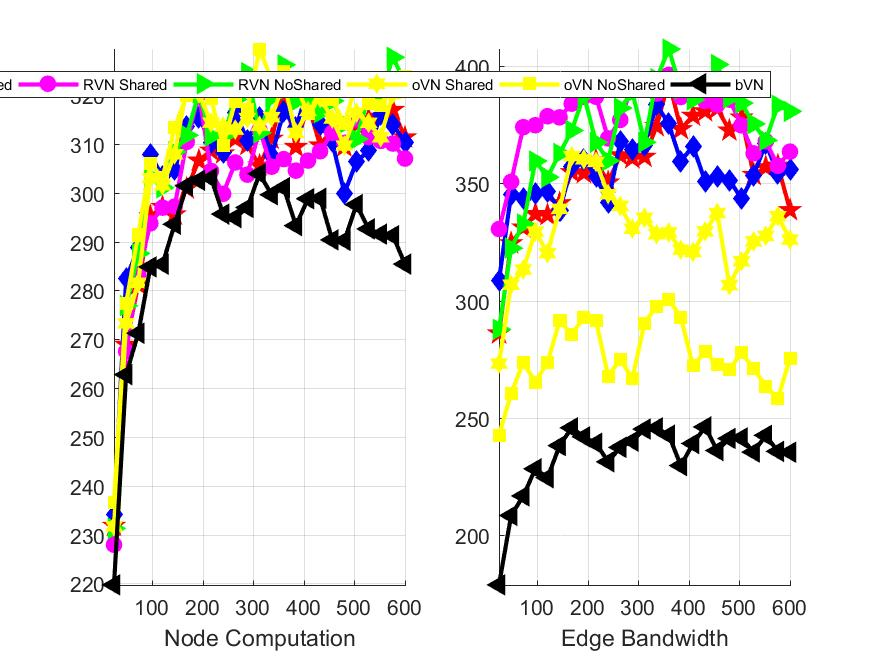
\includegraphics[width=3in]{Fig/CostCurrentSubstrateNetwork}\\
  \caption{Substrate Network Current Cost}\label{fig:CostCurrentSubstrateNetwork}
\end{figure}

Cost Accumulate SubstrateNetwork\ref{fig:CostAccumulateSubstrateNetwork}:
\begin{figure}
  \centering
  % Requires \usepackage{graphicx}
  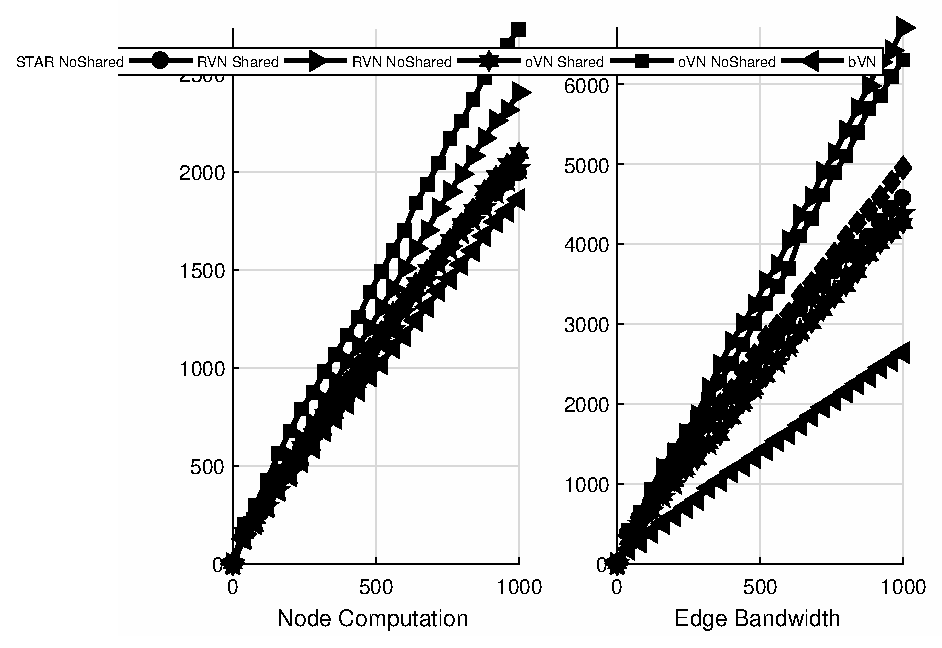
\includegraphics[width=3in]{Fig/CostAccumulateSubstrateNetwork}\\
  \caption{Substrate Network Accumulate Cost}\label{fig:CostAccumulateSubstrateNetwork}
\end{figure}

Cost Average Current Substrate Network\ref{fig:CostAverageCurrentSubstrateNetwork}:
\begin{figure}
  \centering
  % Requires \usepackage{graphicx}
  \includegraphics[width=3in]{Fig/CostAverageCurrentSubstrateNetwork}\\
  \caption{Substrate Network Current Average Cost}\label{fig:CostAverageCurrentSubstrateNetwork}
\end{figure}

Cost Average Accumulate SubstrateNetwork\ref{fig:CostAverageAccumulateSubstrateNetwork}:
\begin{figure}
  \centering
  % Requires \usepackage{graphicx}
  \includegraphics[width=3in]{Fig/CostAverageAccumulateSubstrateNetwork}\\
  \caption{Substrate Network Accumulate Average Cost }\label{fig:CostAverageAccumulateSubstrateNetwork}
\end{figure}



\subsection{Revenue}
Revenue: Sum of CPU and bandwidth demands realized for the virtual networks.

Revenue Current Virtual Network\ref{fig:RevenueCurrentVirtualNetwork}:
\begin{figure}
  \centering
  % Requires \usepackage{graphicx}
  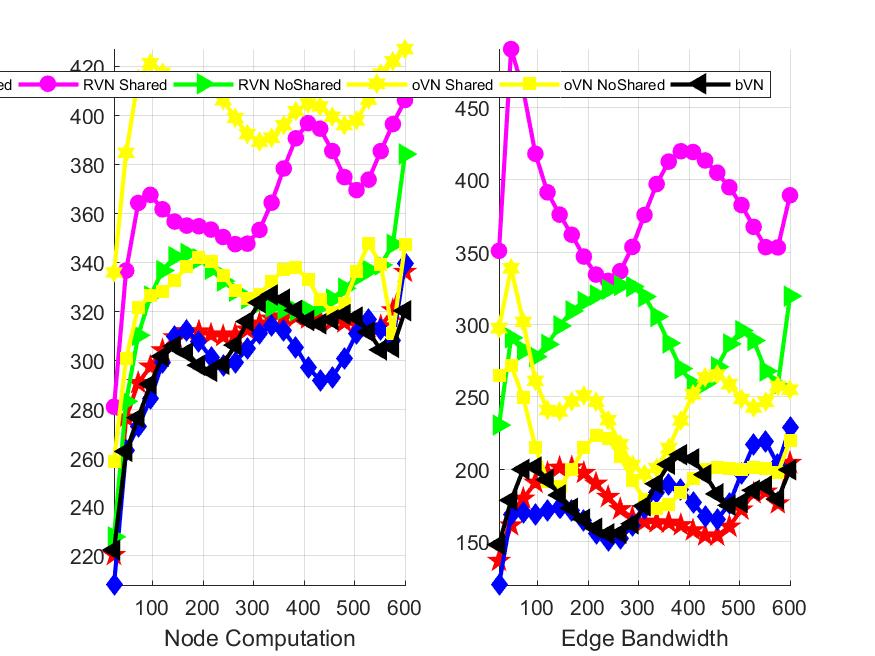
\includegraphics[width=3in]{Fig/RevenueCurrentVirtualNetwork}\\
  \caption{Virtual Network Current Revenue }\label{fig:RevenueCurrentVirtualNetwork}
\end{figure}

Revenue Accumulate Virtual Network\ref{fig:RevenueAccumulateVirtualNetwork}:
\begin{figure}
  \centering
  % Requires \usepackage{graphicx}
  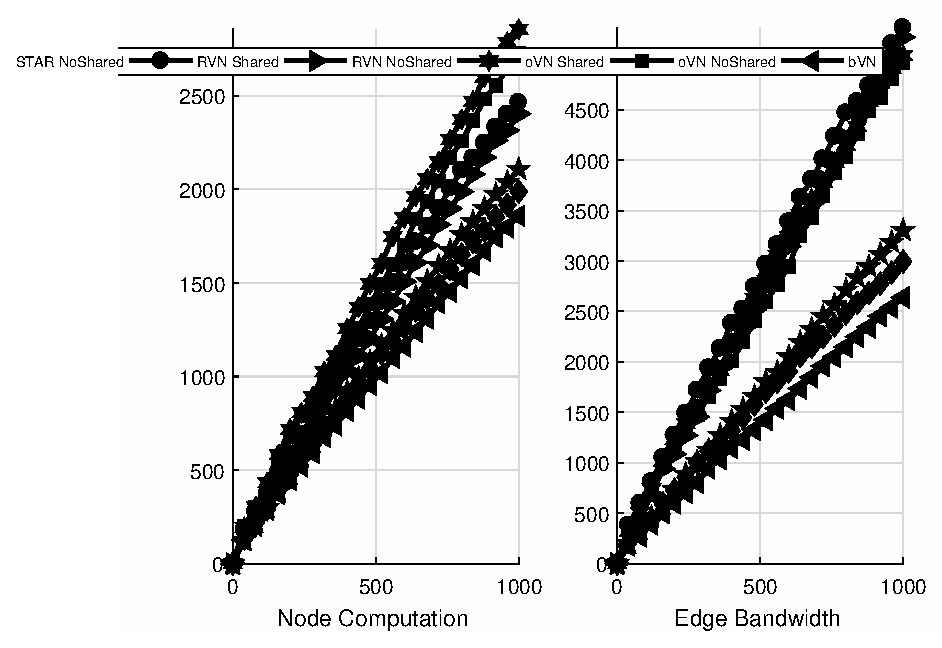
\includegraphics[width=3in]{Fig/RevenueAccumulateVirtualNetwork}\\
  \caption{Virtual Network Accumulate Revenue }\label{fig:RevenueAccumulateVirtualNetwork}
\end{figure}

Revenue Average Current Virtual Network\ref{fig:RevenueAverageCurrentVirtualNetwork}:
\begin{figure}
  \centering
  % Requires \usepackage{graphicx}
  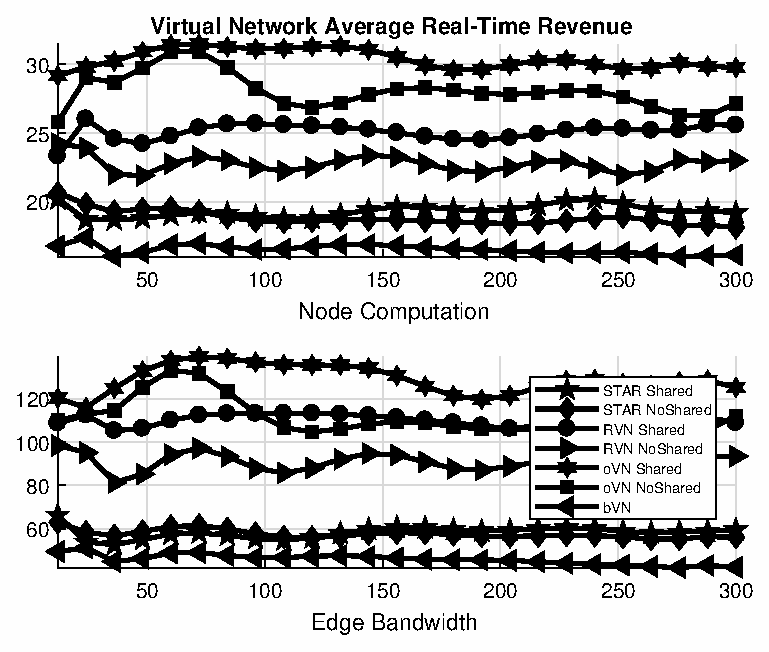
\includegraphics[width=3in]{Fig/RevenueAverageCurrentVirtualNetwork}\\
  \caption{Virtual Network Current Average Revenue}\label{fig:RevenueAverageCurrentVirtualNetwork}
\end{figure}

Revenue Average Accumulate Virtual Network\ref{fig:RevenueAverageAccumulateVirtualNetwork}:
\begin{figure}
  \centering
  % Requires \usepackage{graphicx}
  \includegraphics[width=3in]{Fig/RevenueAverageAccumulateVirtualNetwork}\\
  \caption{Virtual Network Accumulate Average Revenue}\label{fig:RevenueAverageAccumulateVirtualNetwork}
\end{figure}


\subsection{Cost/Revenue}
Cost/Revenue: The ratio indicates the virtualization overhead.

Cost/Revenue\ref{fig:CostRevenue}:
\begin{figure}
  \centering
  % Requires \usepackage{graphicx}
  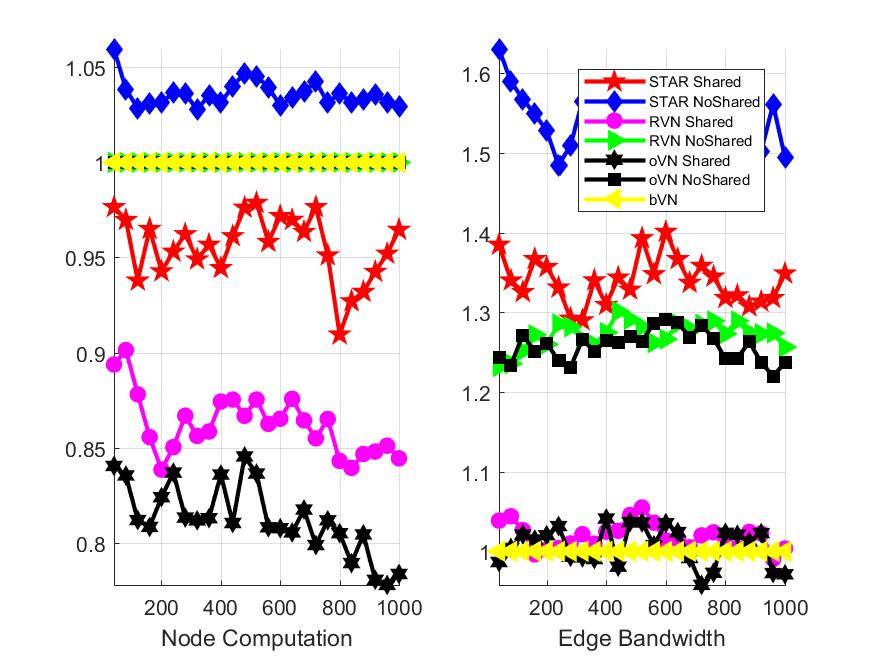
\includegraphics[width=3in]{Fig/CostRevenue}\\
  \caption{Cost/Revenue}\label{fig:CostRevenue}
\end{figure}

Cost Revenue Accumulate\ref{fig:CostRevenueAccumulate}:
\begin{figure}
  \centering
  % Requires \usepackage{graphicx}
  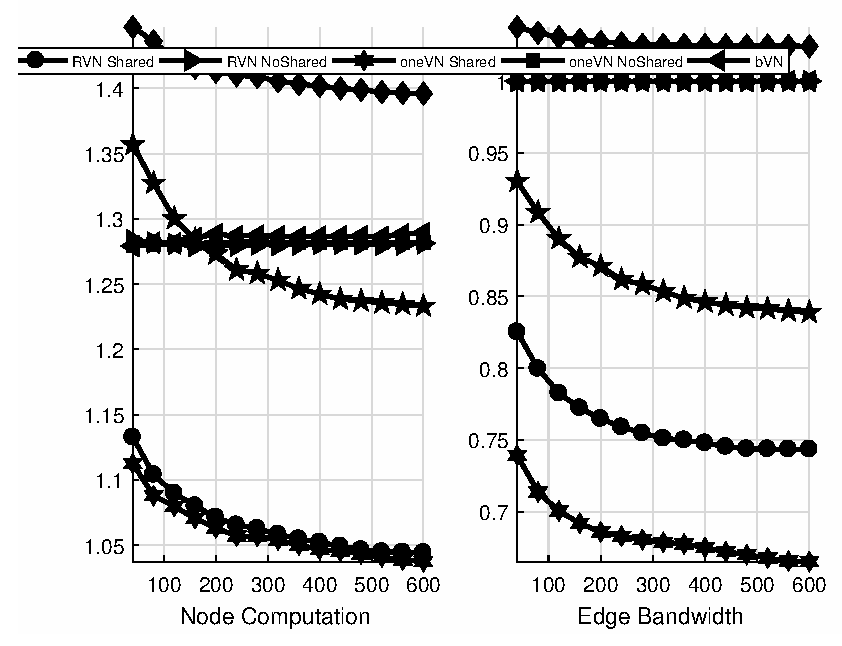
\includegraphics[width=3in]{Fig/CostRevenueAccumulate}\\
  \caption{Accumulate Cost Revenue}\label{fig:CostRevenueAccumulate}
\end{figure}

\subsection{Virtual Network Request and successful Survivable embedded Virtual Network Request}
\begin{figure}
  \centering
  % Requires \usepackage{graphicx}
  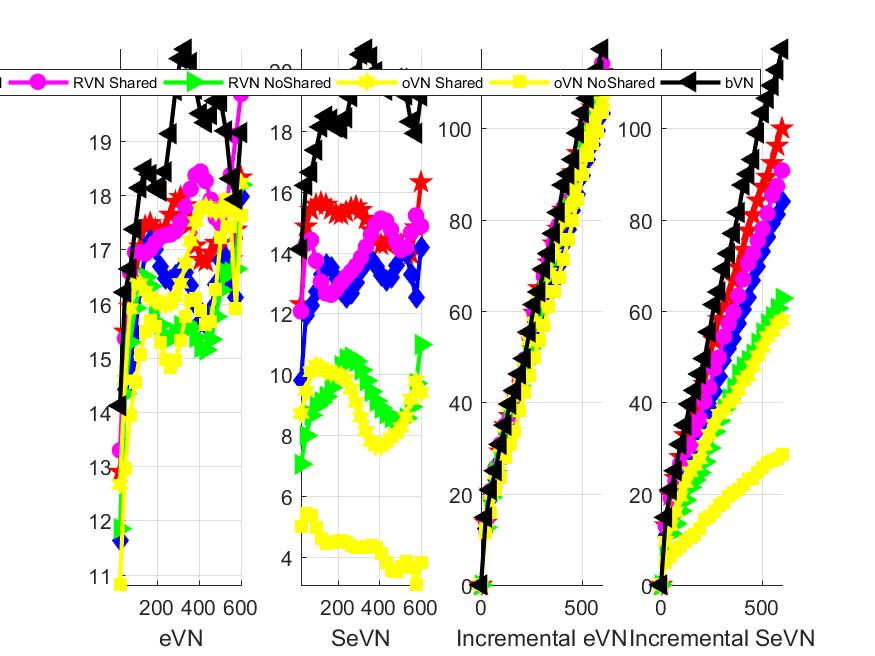
\includegraphics[width=3in]{Fig/VirNetReqSurNetReq}\\
  \caption{Virtual Network Request and successful Survivable embedded Virtual Network Request}\label{fig:VirNetReqSurNetReq}
\end{figure}

\subsection{Migration Frequency}
\begin{figure}
  \centering
  % Requires \usepackage{graphicx}
  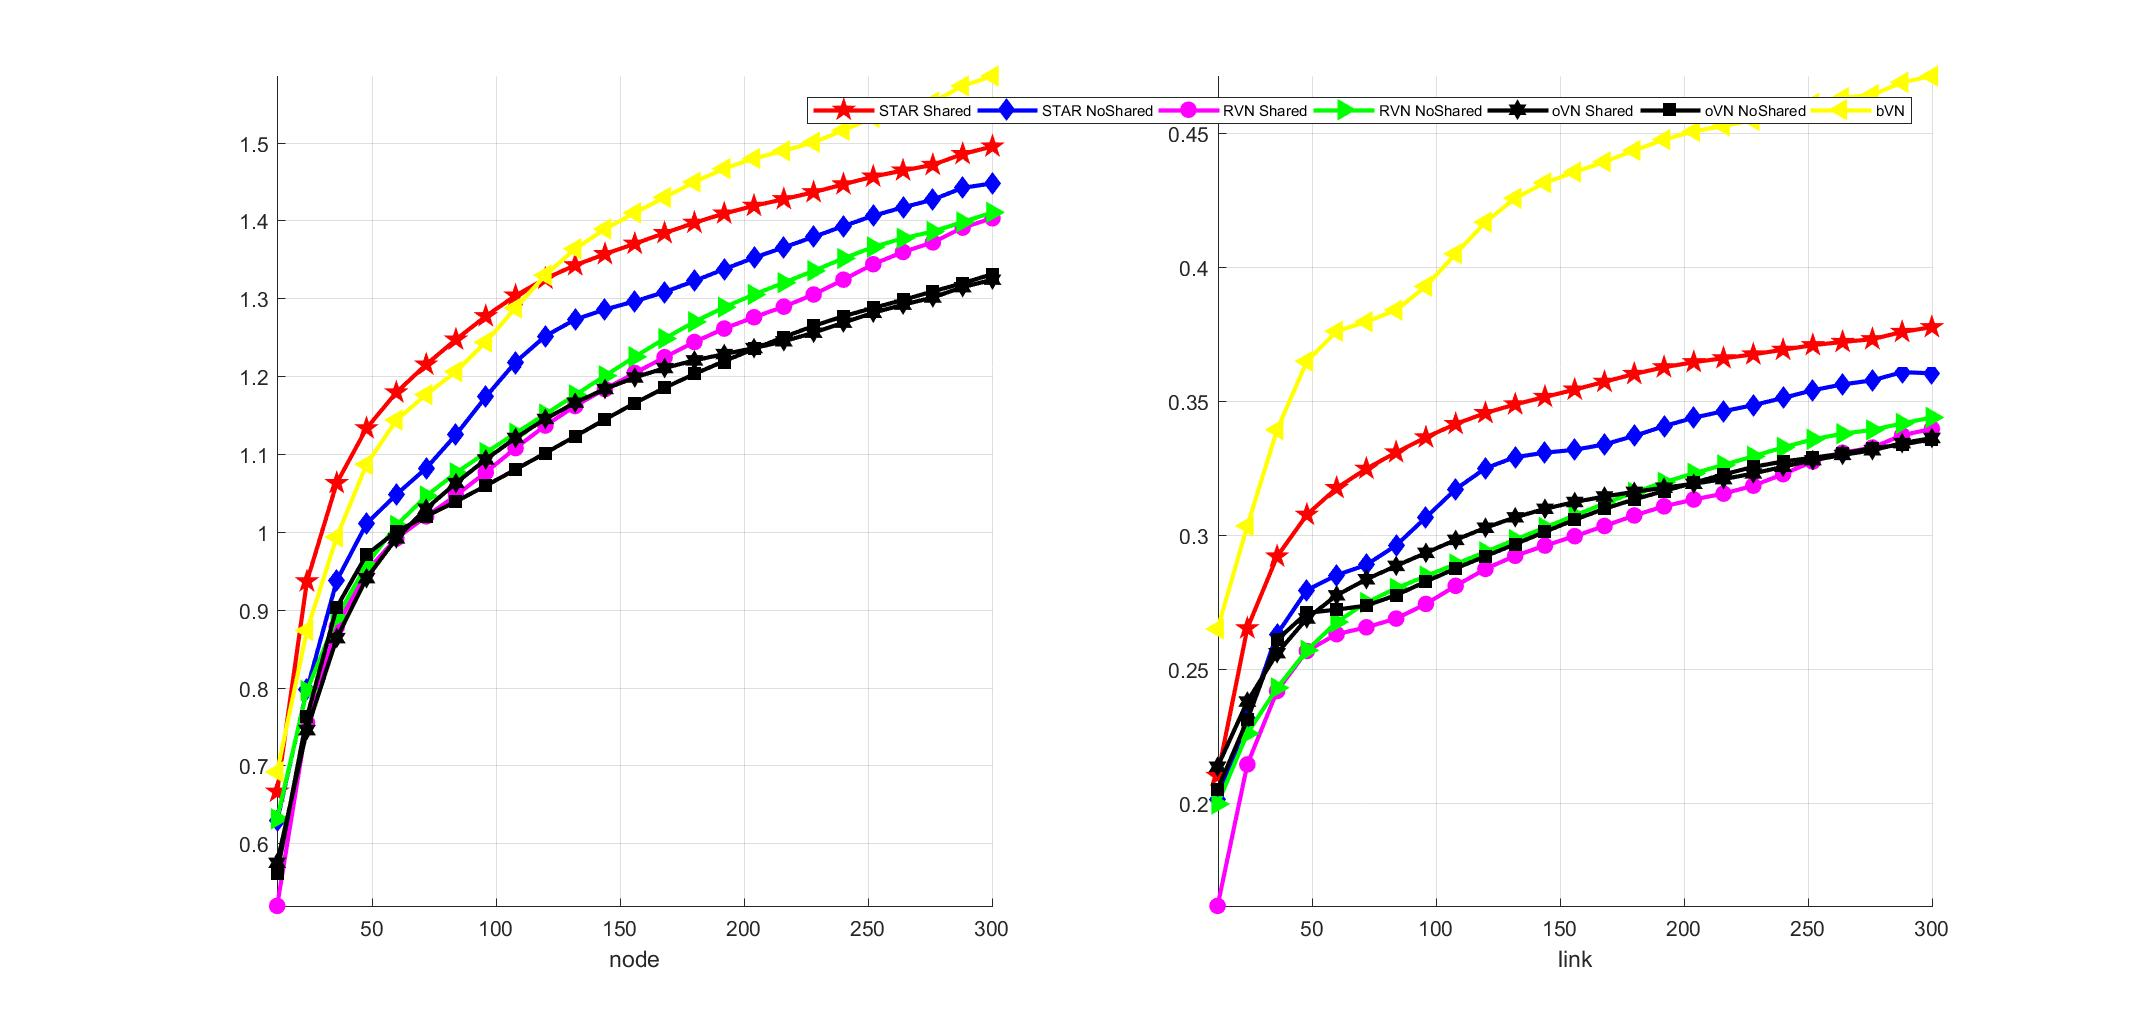
\includegraphics[width=3in]{Fig/MigrationFrequence}\\
  \caption{Migration Frequency Ratio}\label{fig:MigrationFrequence}
\end{figure}
%As mentioned above, FD-EVN algorithms achieve higher acceptance ratio and lower embedding cost at the cost of more node migration after facility node failure, which would cause service interruption and should be examined carefully, especially for the application with SLA constraints. We run our simulation in $\SubstrateNewtorkRunTimeInterval$ time unites, which corresponds to about $\SubStrateFacilityNodeFailDuration$ requests on average in each instance of simulation. The migration frequency
%after random facility node  failure is presented in Fig. 8 in terms of the number of VN nodes.


%\begin{figure*}
%  \centering
%  % Requires \usepackage{graphicx}
%
%
%
% \begin{equation*}
%\left[ {\begin{array}{*{20}{c}}
%&C_{P_{2.2}}&C_{P_{2.3}}&C_{P_3}&C_{P_4}&C_{B_{1.1}}&C_{B_{1.2}}&C_{B_{2.1}}&C_{B_{2.4}}&C_{B_{3.2}}&C_{B_{3.2}}\\
%{R_{V_1}}&\infty&\infty&\infty&\infty&\fbox{N+(2)+4+5+3}&\infty&${N+(2)+4+5+3}$&\infty&\infty&\infty\\
%R_{V_2}&\fbox{4}&\infty&\infty&\infty&\infty&${N+(3)+4+6}$&\infty&\infty&${N+(3)+4+6}$&\infty\\
%R_{V_3}&\infty&${M+(2)+5}$&\fbox{5}&\infty&\infty&\infty&\infty&\infty&\infty&${N+(5)+5+6}$\\
%R_{V_4}&\infty&\infty&\infty&\fbox{3}&\infty&\infty&\infty&${N+(6)+3}$&\infty&\infty\\
%\end{array}} \right]
%\end{equation*}
% \begin{equation*}
%\left[ {\begin{array}{*{20}{c}}
%&C_{P_{1}}&C_{P_3}&C_{P_4}&C_{B_{1.1}}&C_{B_{1.2}}&C_{B_{2.1}}&C_{B_{2.4}}&C_{B_{3.2}}&C_{B_{3.2}}\\
%{R_{V_1}}&4&\infty&\infty&${M+4}$&\infty&$N+(2)+4+5+3$&\infty&\infty&\infty\\
%R_{V_2}&\infty&\infty&\infty&\infty&${M+(1)+4+1} $&\infty&\infty&${N+(3)+4+6}$&\infty\\
%R_{V_3}&\infty&6&\infty&\infty&\infty&\infty&\infty&\infty&$N+(5)+5+6$\\
%R_{V_4}&\infty&\infty&0&\infty&\infty&\infty&$N+(6)+3$&\infty&\infty\\
%\end{array}} \right]
%\end{equation*}
%
% \begin{equation*}
%\left[ {\begin{array}{*{20}{c}}
%&C_{P_{1}}&C_{P_{2.2}}&C_{P_{2.3}}&C_{P_4}&C_{B_{1.1}}&C_{B_{1.2}}&C_{B_{2.1}}&C_{B_{2.4}}&C_{B_{3.2}}&C_{B_{3.3}}\\
%R_{V_1}&\fbox{5}&\infty&\infty&\infty&M+5&\infty&${N+(2)+4+5+3}$&\infty&\infty&\infty\\
%R_{V_2}&\infty&\mbox{6}&\infty&\infty&\infty&\fbox{M+6}&\infty&\infty&${N+(3)+4+6}$&\infty\\
%R_{V_3}&\infty&\infty&\fbox{M+(2)+1}&\infty&\infty&\infty&\infty&\infty&\infty&${N+(5)+5+6}$\\
%R_{V_4}&\infty&\infty&\infty&\fbox{0}&\infty&\infty&\infty&${N+(6)+3}$&\infty&\infty\\
%\end{array}} \right]
%\end{equation*}
%\end{figure*}





%\end{CJK*}

%\appendix
%This appendix will try to clarify themain differences between
%the considered heuristics. The network which will be used
